% Drawing 156-8/05-2 -- folder 156-8, batch 05, archive page 97 (PDF page 98).
% Transcription: un segment horizontal découpé en intervalles par des points marqués $t_1, t_2, t_3, \ldots, t_{n-1}, t_n$.
% Kind: subdivided segment. Method 3 (encoded, rendered from the data). Status: ok.
% Notes: A horizontal segment cut into intervals by the points t1, t2, t3, ..., t_{n-1}, t_n; the stretch after t3 is dotted. Encoded as segment-config/1 (points and intervals, left to right).
% Coordinates: 1 unit = 1 mm = 1/100 of the crop width (bbox in page fractions: [0.25, 0.23, 0.75, 0.31]).
% Redrawn by Claude (claude-opus-5-5), issue #73 pilot, 2026-11-07; not checked by a human; not compiled (no TeX in the session).
% Rights: reproduces part of the work -- behind RENDER_TRANSCRIPTS, never published by itself.
\documentclass[tikz,border=3pt]{standalone}
\usepackage{amsmath,amssymb}
\usetikzlibrary{patterns,arrows.meta}
\tikzset{pencil/.style={black!45}, struck/.style={black!35}, mark/.style={circle,draw,inner sep=1.3pt}, pt/.style={circle,fill,inner sep=0.9pt}, opt/.style={circle,draw,fill=white,inner sep=1.1pt}}
\begin{document}
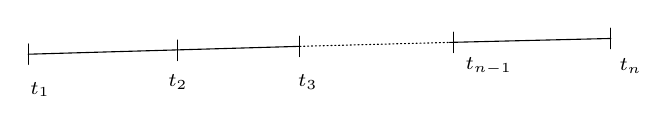
\begin{tikzpicture}[x=1mm,y=1mm,line cap=round,line join=round,font=\scriptsize]
\draw (10.5,-14) -- (45,-13);
\draw[densely dotted] (45,-13) -- (64,-12.5);
\draw (64,-12.5) -- (84.5,-12);
\draw (10.5,-12.7) -- (10.5,-15.3);
\draw (29.5,-12.2) -- (29.5,-14.8);
\draw (45,-11.7) -- (45,-14.3);
\draw (64.5,-11.2) -- (64.5,-13.8);
\draw (84.5,-10.7) -- (84.5,-13.3);
\node[inner sep=1pt] at (12,-18.5) {\scriptsize $t_1$};
\node[inner sep=1pt] at (29.5,-17.5) {\scriptsize $t_2$};
\node[inner sep=1pt] at (46,-17.5) {\scriptsize $t_3$};
\node[inner sep=1pt] at (69,-15.5) {\scriptsize $t_{n-1}$};
\node[inner sep=1pt] at (87,-15.5) {\scriptsize $t_n$};
\end{tikzpicture}
\end{document}
